\externaldocument{chapter2}
\chapter{Обучение нейросети} \label{ch3}

% не рекомендуется использовать отдельную section <<введение>> после лета 2020 года
%\section{Введение} \label{ch3:intro}

В данной главе будет представлено описание данных с примерами, а также будет рассказано о процессе обучения предлагаемой нейросети и его результатах.

\section{Данные для обучения} \label{ch3:sec1}
Для обучения и тестирования нейросети использовался набор данных (датасет) из открытых источников \cite{jiang2018transform}. В нем представлено более 900 тыс. снимков различных типов объектов с микроскопа разного разрешения и с разным числом каналов. Для обучения нейросети будут использоваться 14 тыс. изображений клеток, отснятых на 20-кратном увеличении. Глубина резкости используемого объектива равна 1 мкм. Данные представлены в виде набора файлов (изображений в формате jpeg) с именами <<defocus[N]>>, где N -- число со знаком, означающее отклик, который нужно предсказать. Например, имя файла <<defocus-550.jpg>> означает, что текущая плоскость, на которой фокусируется камера, находится на расстоянии -550 нанометров. Число -550 -- это то значение, которое должно получиться в качестве результата работы нейросети. Пример входных данных представлен на \firef{fig:data_axample}

\begin{figure}[!htbp]
	\begin{subfigure}[t]{0.45\linewidth}
		\centering
		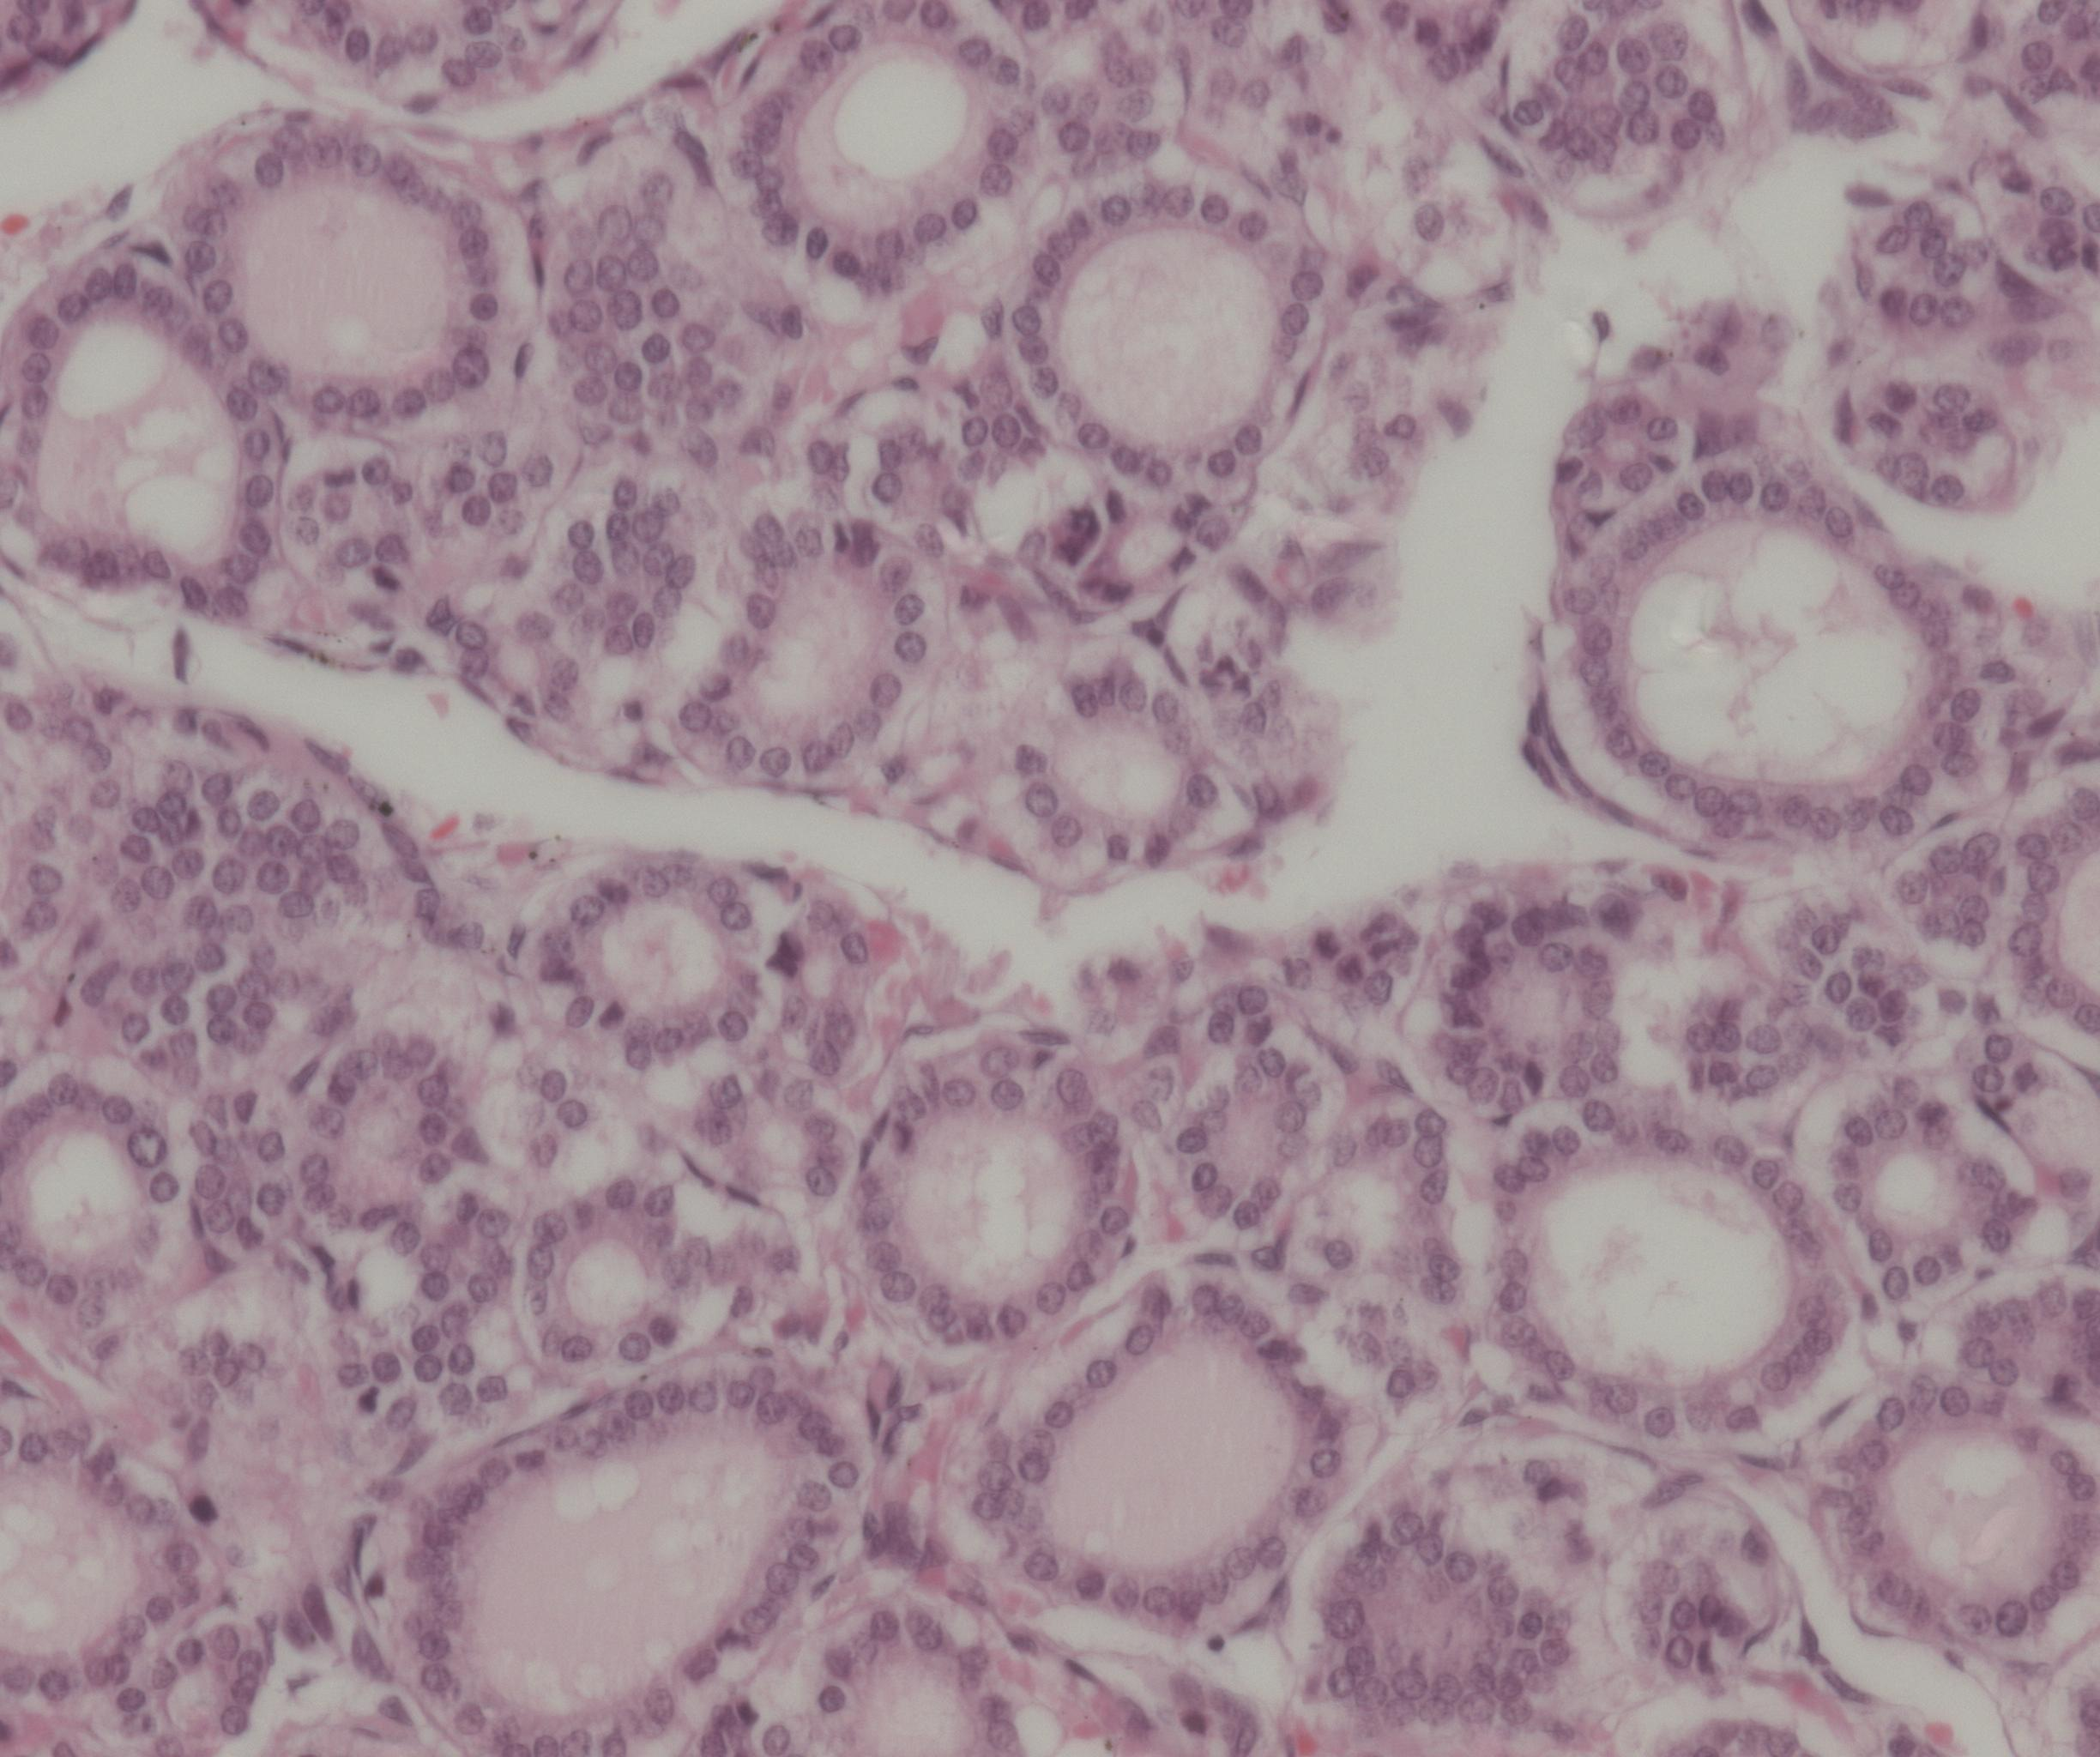
\includegraphics[width=.95\linewidth]{my_folder/images/defocus-550.jpg}
		\caption{}
		\label{fig:data_axample_defocus-550}
	\end{subfigure}
	\hfill
	\begin{subfigure}[t]{0.45\linewidth}
		\centering
		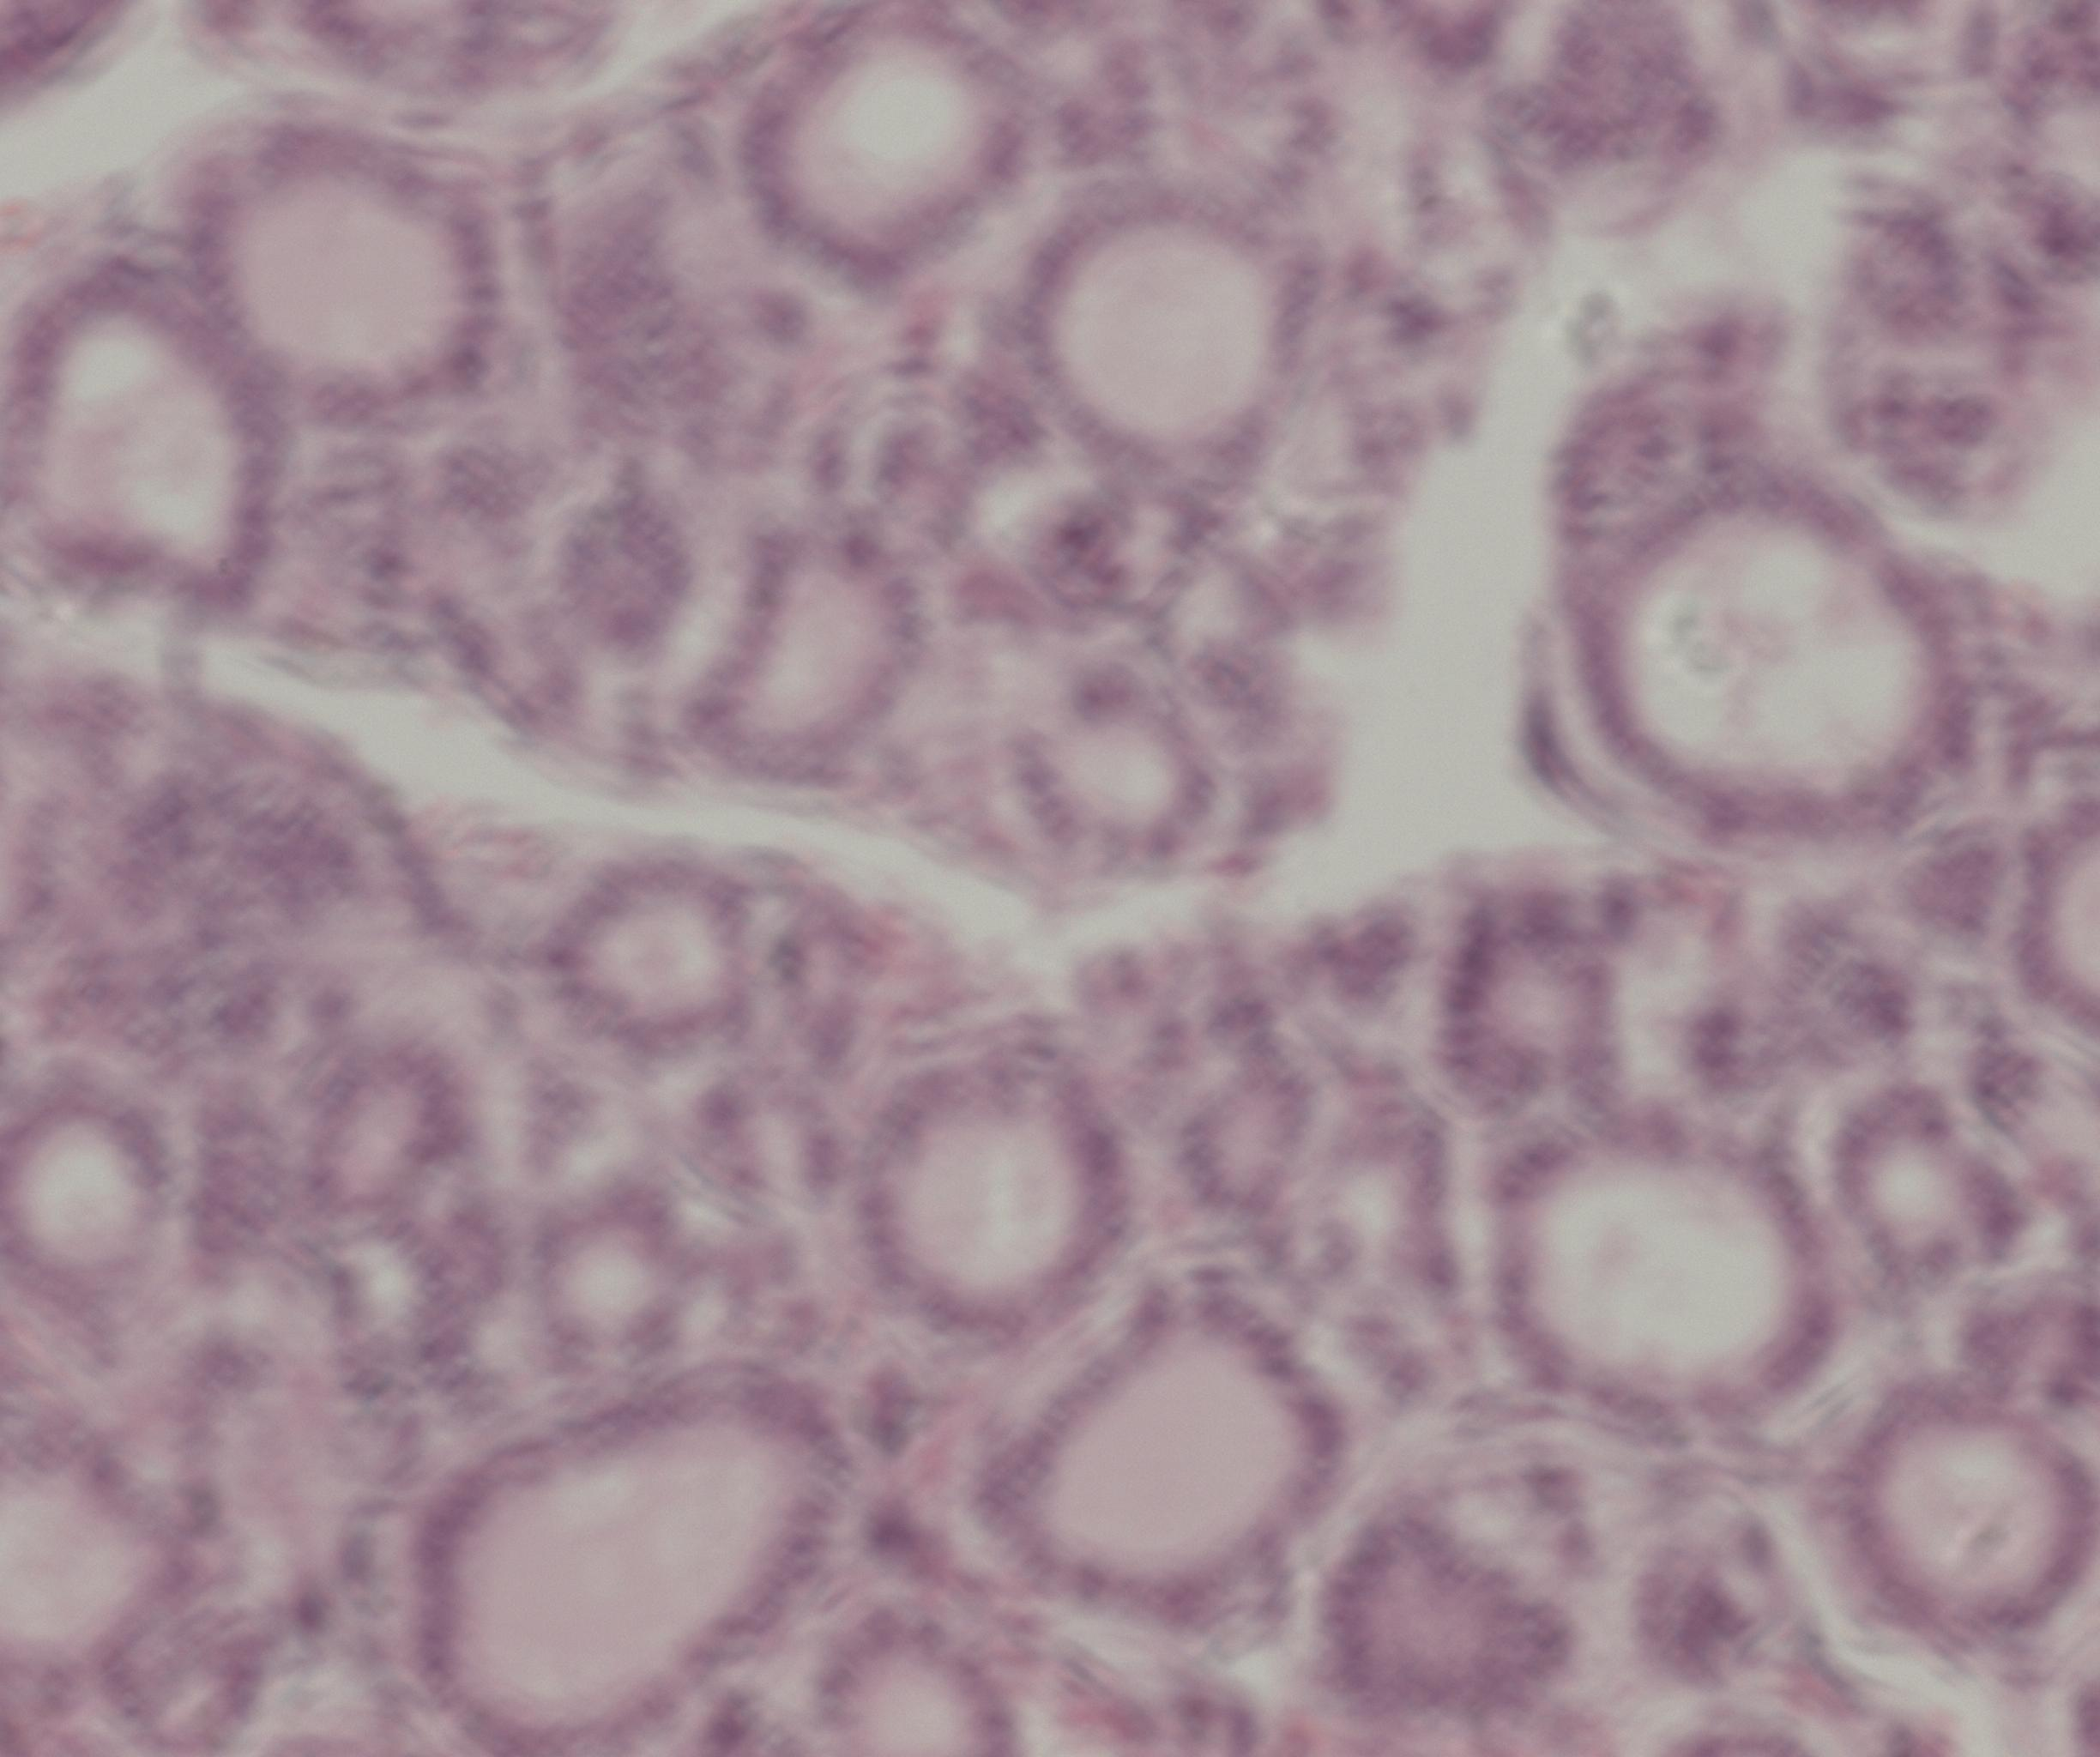
\includegraphics[width=.95\linewidth]{my_folder/images/defocus9950.jpg}
		\caption{}
		\label{fig:data_axample_defocus9550}
	\end{subfigure}
	\caption{Примеры изображений из набора данных: {\itshape a} --- Расстояние дефокусировки -550 нм; {\itshape b} --- Расстояние дефокусировки 9550 нм}
	\label{fig:data_axample}
\end{figure}

Реальные отснятые данные также подтверждают тезис о том, что из-за асимметричности ФРТ изображения на равном расстоянии, но по разные стороны от фокальной плоскости объекта будут различаться (\firef{fig:PSF_example})

\begin{figure}[!htbp]
	\begin{subfigure}[t]{0.45\linewidth}
		\centering
		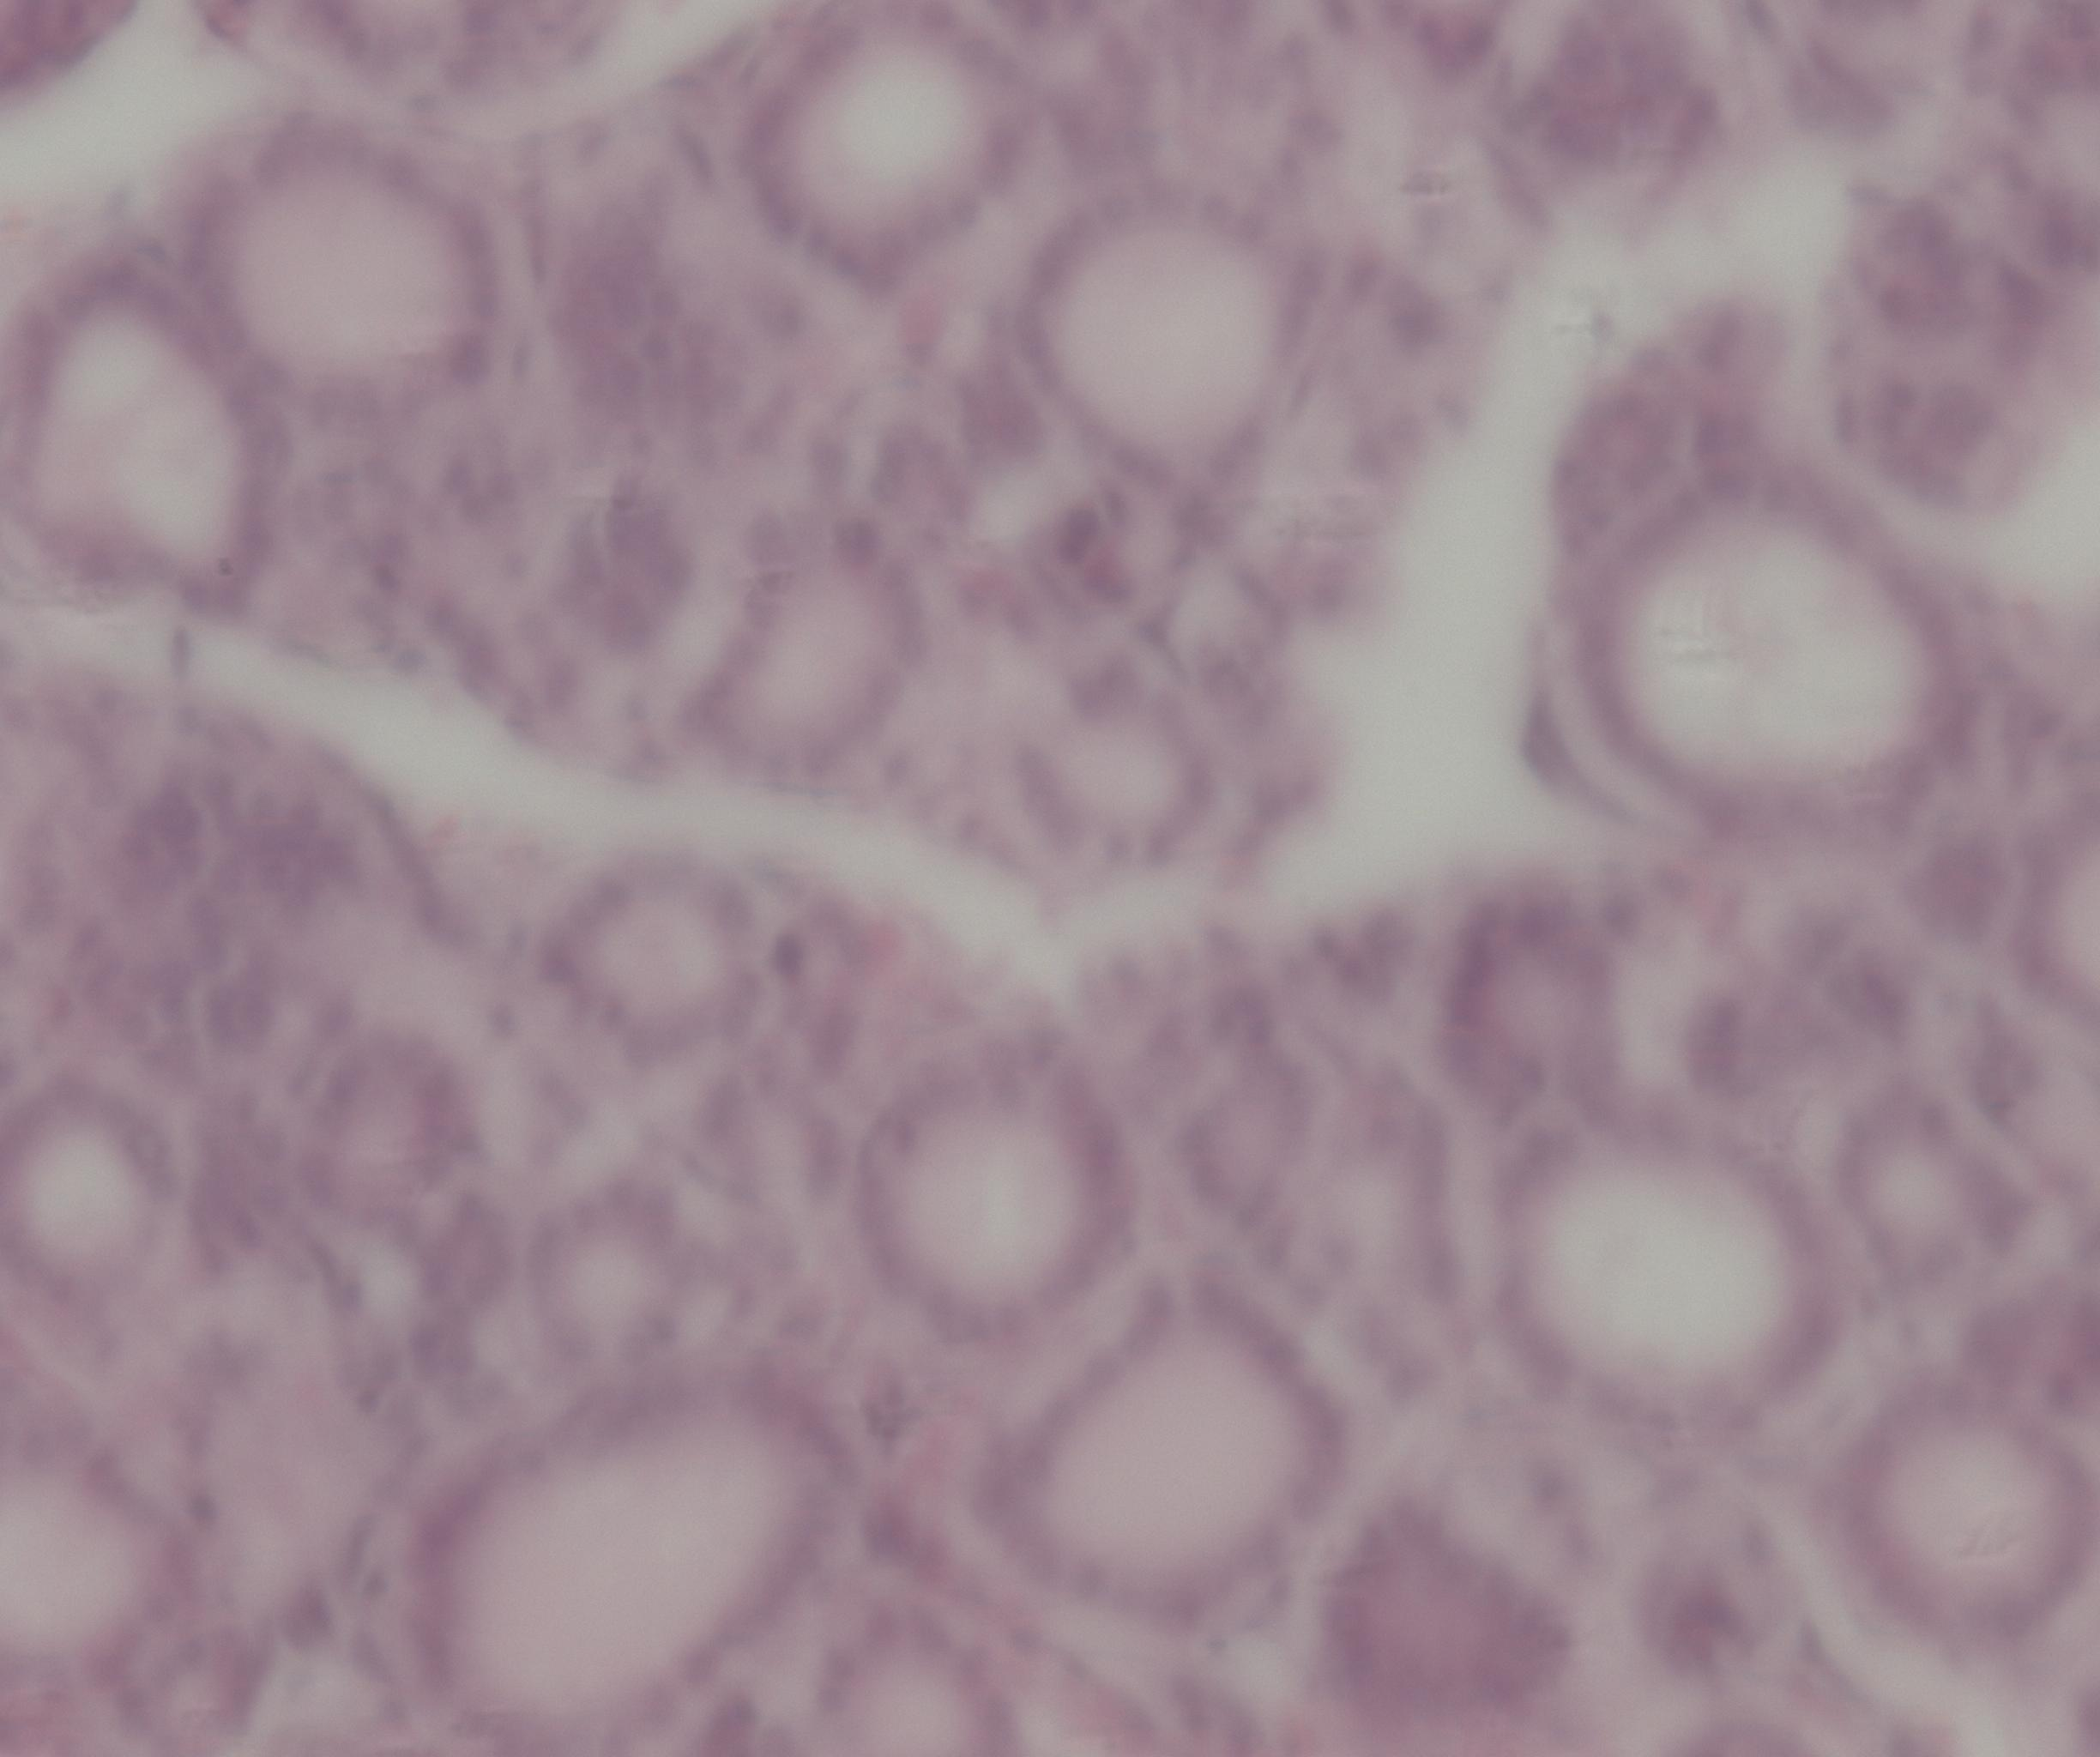
\includegraphics[width=.95\linewidth]{my_folder/images/defocus-9550.jpg}
		\caption{}
		\label{fig:PSF_defocus-9550}
	\end{subfigure}
	\hfill
	\begin{subfigure}[t]{0.45\linewidth}
		\centering
		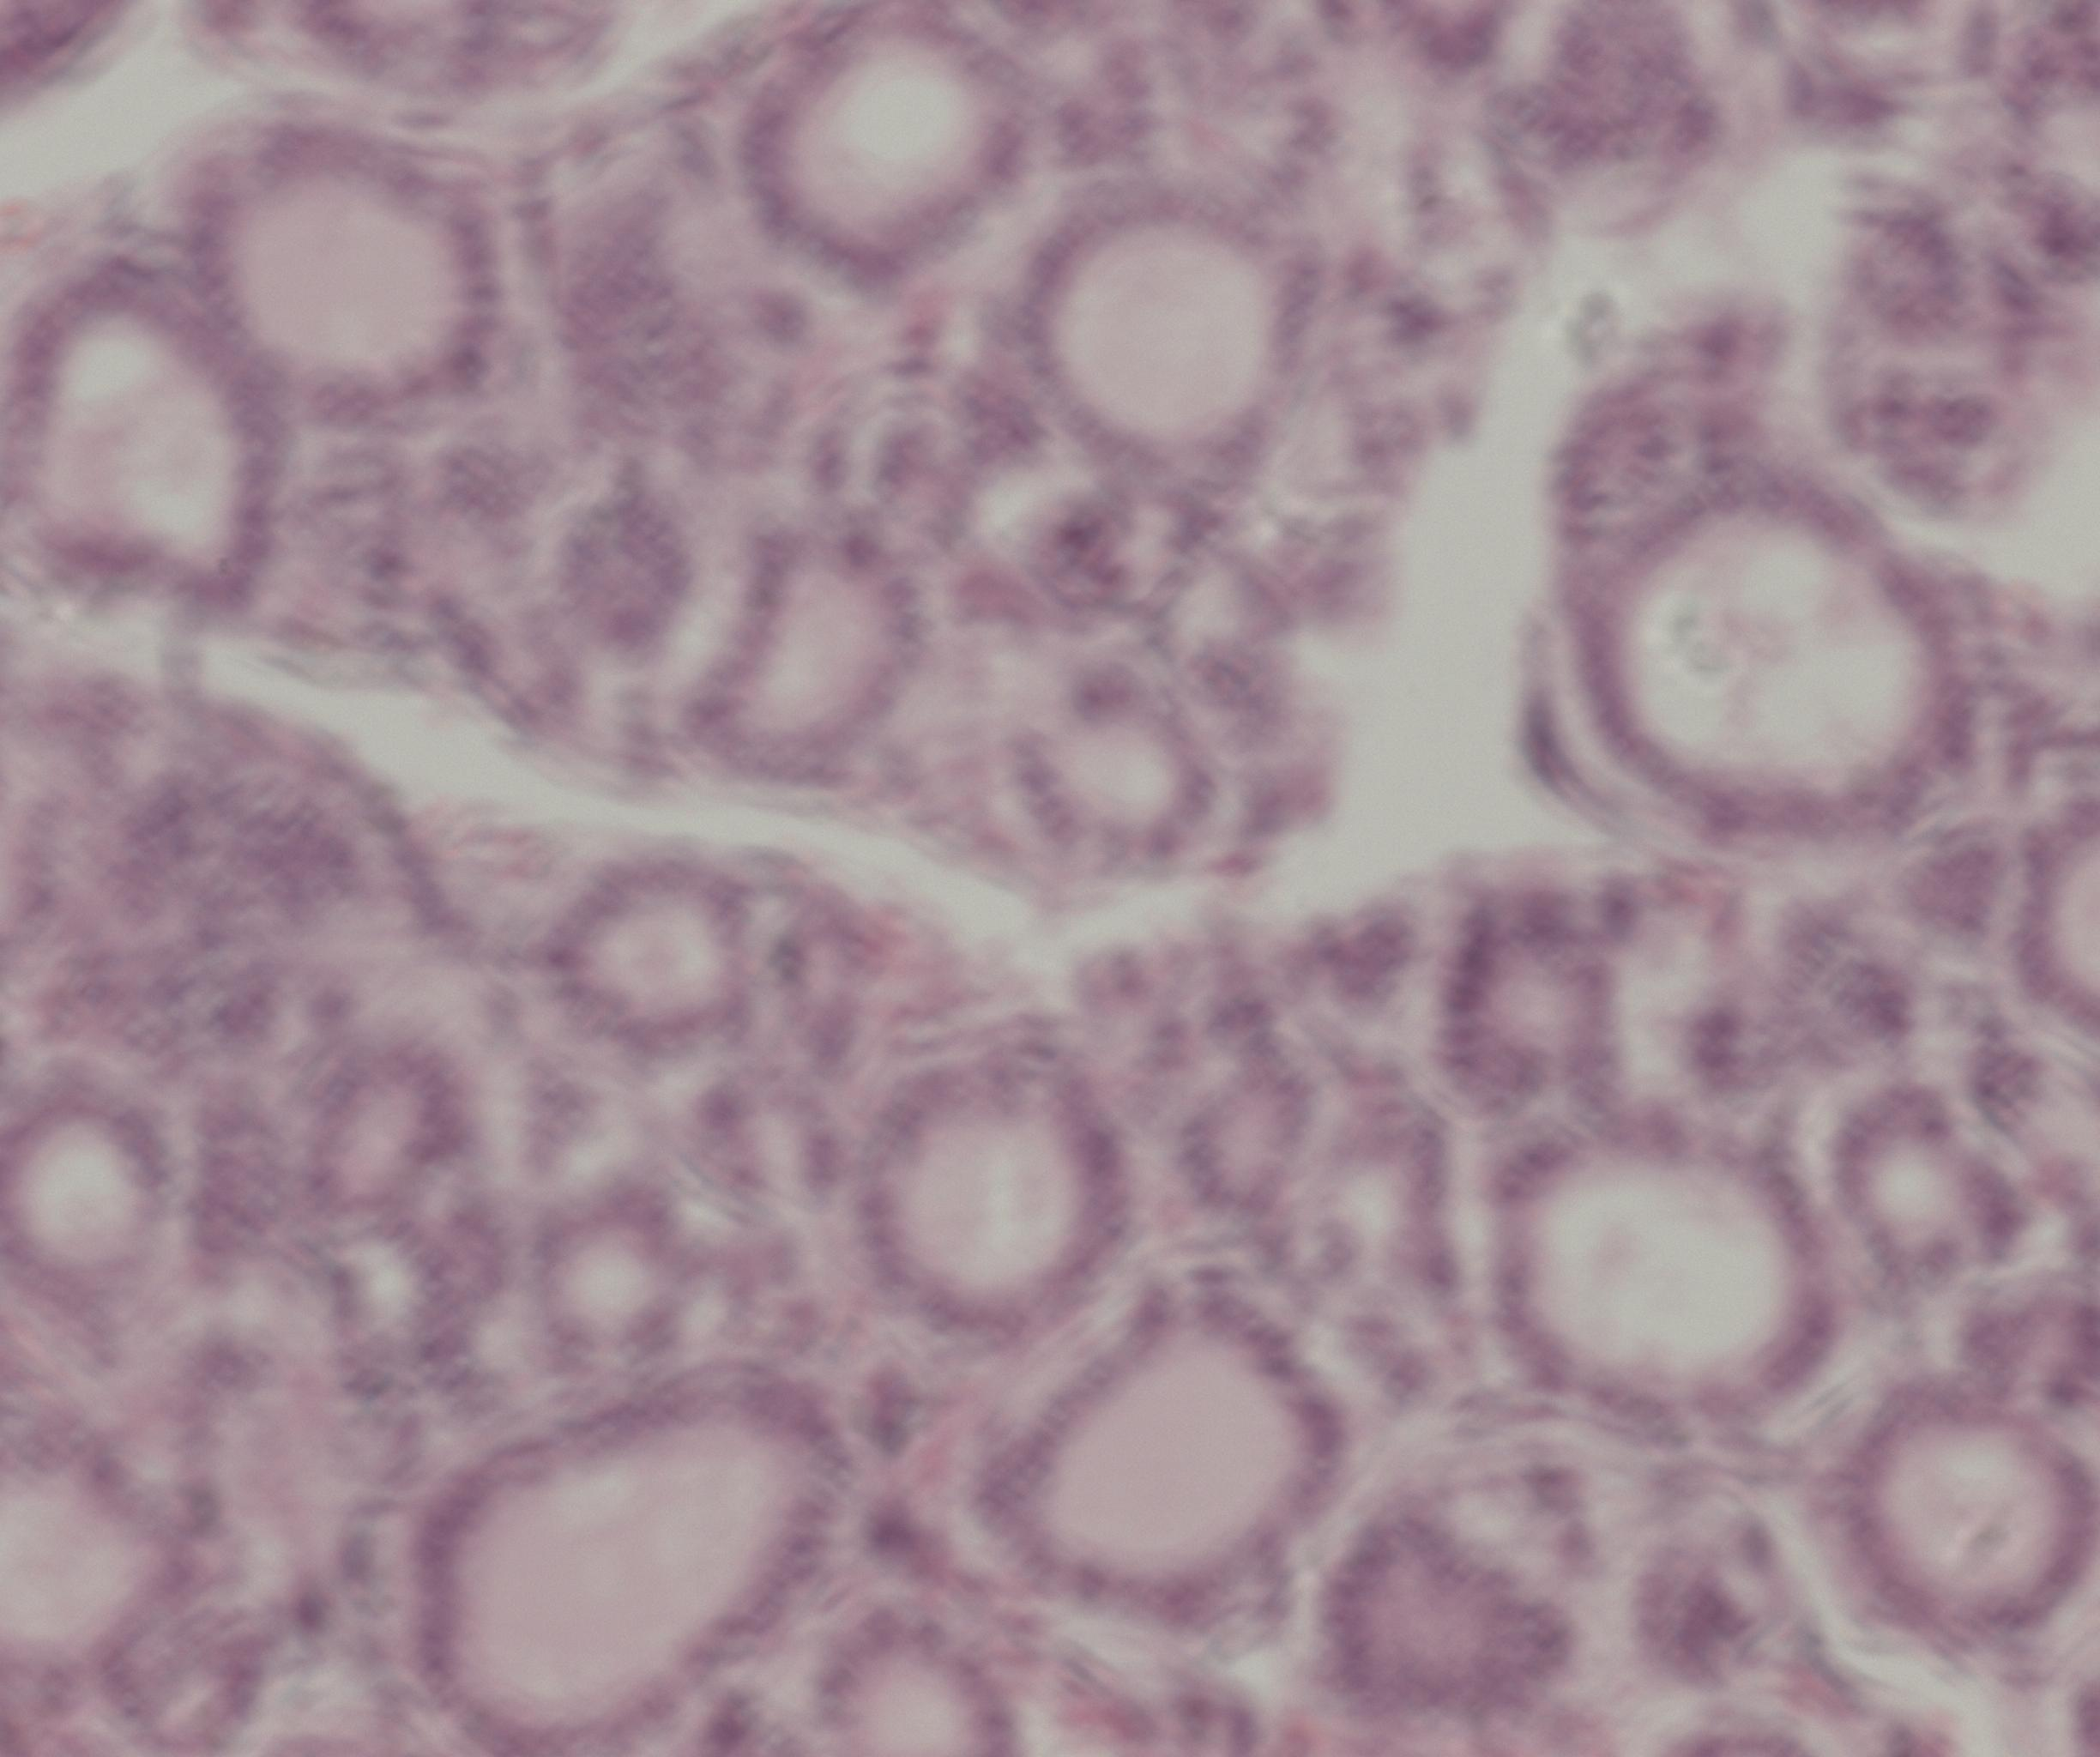
\includegraphics[width=.95\linewidth]{my_folder/images/defocus9950.jpg}
		\caption{}
		\label{fig:PSF_defocus9550}
	\end{subfigure}
	\caption{Примеры асимметрии ФРТ: {\itshape a} --- Расстояние дефокусировки -9550 нм; {\itshape b} --- Расстояние дефокусировки 9550 нм}
	\label{fig:PSF_example}
\end{figure}

\section{Результаты обучения} \label{ch3:sec2}
Набор данных был разделен на тренировочную, валидационную и тестовую выборки в соотношении 80:10:10.

\textit{Тренировочная выборка} -- часть набора данных, используемая для обучения модели, то есть для настройки весов и других обучаемых параметров ее слоев.

\textit{Валидационная выборка} -- данные, которые также используются в процессе обучения, но не влияют на обучаемые параметры. Валидационная выборка используется для корректировки гиперпараметров модели.

\textit{Тестовая выборка} -- данные, которые первый раз подаются на вход нейронной сети только после полного процесса обучения. Она используется для оценки качества модели на новых, незнакомых ей данных.

Обучение (или тренировка) производилось на графическом процессоре NVIDIA GeForce RTX 2080Ti с 11 Гб видеопамяти. Для ускорения обучения использовалась подача изображений пакетами (batch) по 30 штук. Тренировка проходила в течение 200 эпох, скорость обучения (learning rate) была динамической с начальным значением 0.001 и уменьшалась в 10 раз, если в течение 5 эпох не происходило улучшение показателей ошибки. Время обучения составляло 13 часов. График оптимизируемой функции представлен на \firef{fig:loss}. 

\begin{figure}[ht] 
	\center
	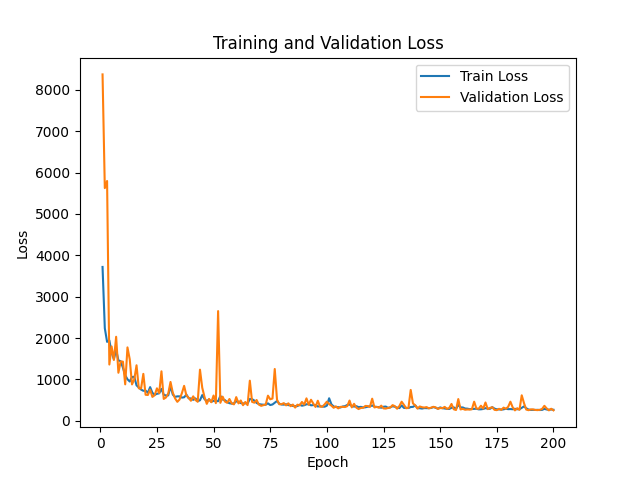
\includegraphics [scale=1.0] {my_folder/images/losses_200_epochs.png}
	\caption{Результат обучения. Ось OX -- номер эпохи, ось OY -- величина функции потерь}
	\label{fig:loss}
\end{figure}

\section{Метрики}
Для обучения нейронной сети и оценки ее качества использовалась функция потерь smooth L1-loss, как было сказано в параграфе \ref{ch2:architecture}. В процессе обучения она минимизируется. Также замеряется время работы алгоритма.

Для оценки результата на тестовом наборе также используется метрика $MAE$:
\begin{equation}
	MAE = \dfrac{1}{N} \sum\limits_{i=1}^N \left|y_i - y'\right|,
\end{equation}

где $y$ -- истинное значение отклика, $y'$ -- предсказанное значение, $N$ -- мощность тестовой выборки.

%\FloatBarrier % заставить рисунки и другие подвижные (float) элементы остановиться


\section{Эксперименты} \label{ch3:experiments}

%На \firef{fig:Result_example} представлен результат работы предложенной нейросети при том же увеличении, что и данные для обучения. Хорошо видно, что изображение стало четче, границы объектов различимые и резкие.

Так как одна из целей работы -- разработка решения, не требующего применения дополнительных датчиков, то прямое сравнение предлагаемой нейронной сети будет проводиться с контрастным автофокусом и методом анализа резкости. Для этого применим эти алгоритмы к одним и тем же данным.

В \taref{tab:Comparison_FocuesNet} представлены средние значения времени работы, ошибки и числа перемещений камеры, необходимого для завершения процесса, для каждого метода. Тестирование производилось на процессоре Intel Core i7-4770 3.4 GHz и видеокарте NVIDIA GeForce RTX 2080Ti. Предлагаемая нейронная сеть имеет более высокую точность. Время расчета одного перемещения у нейросети больше, но, так как дополнительных перемещений камеры не требуется, то общее время работы нейросетевого метода оказывается меньше. Кроме того, средняя ошибка не превосходит половины глубины резкости применяемого объектива (1 мкм), а значит, визуально объект будет находиться в фокусе. 

%\begin{figure}[!htbp]
%	\begin{subfigure}[t]{0.45\linewidth}
%		\centering
%		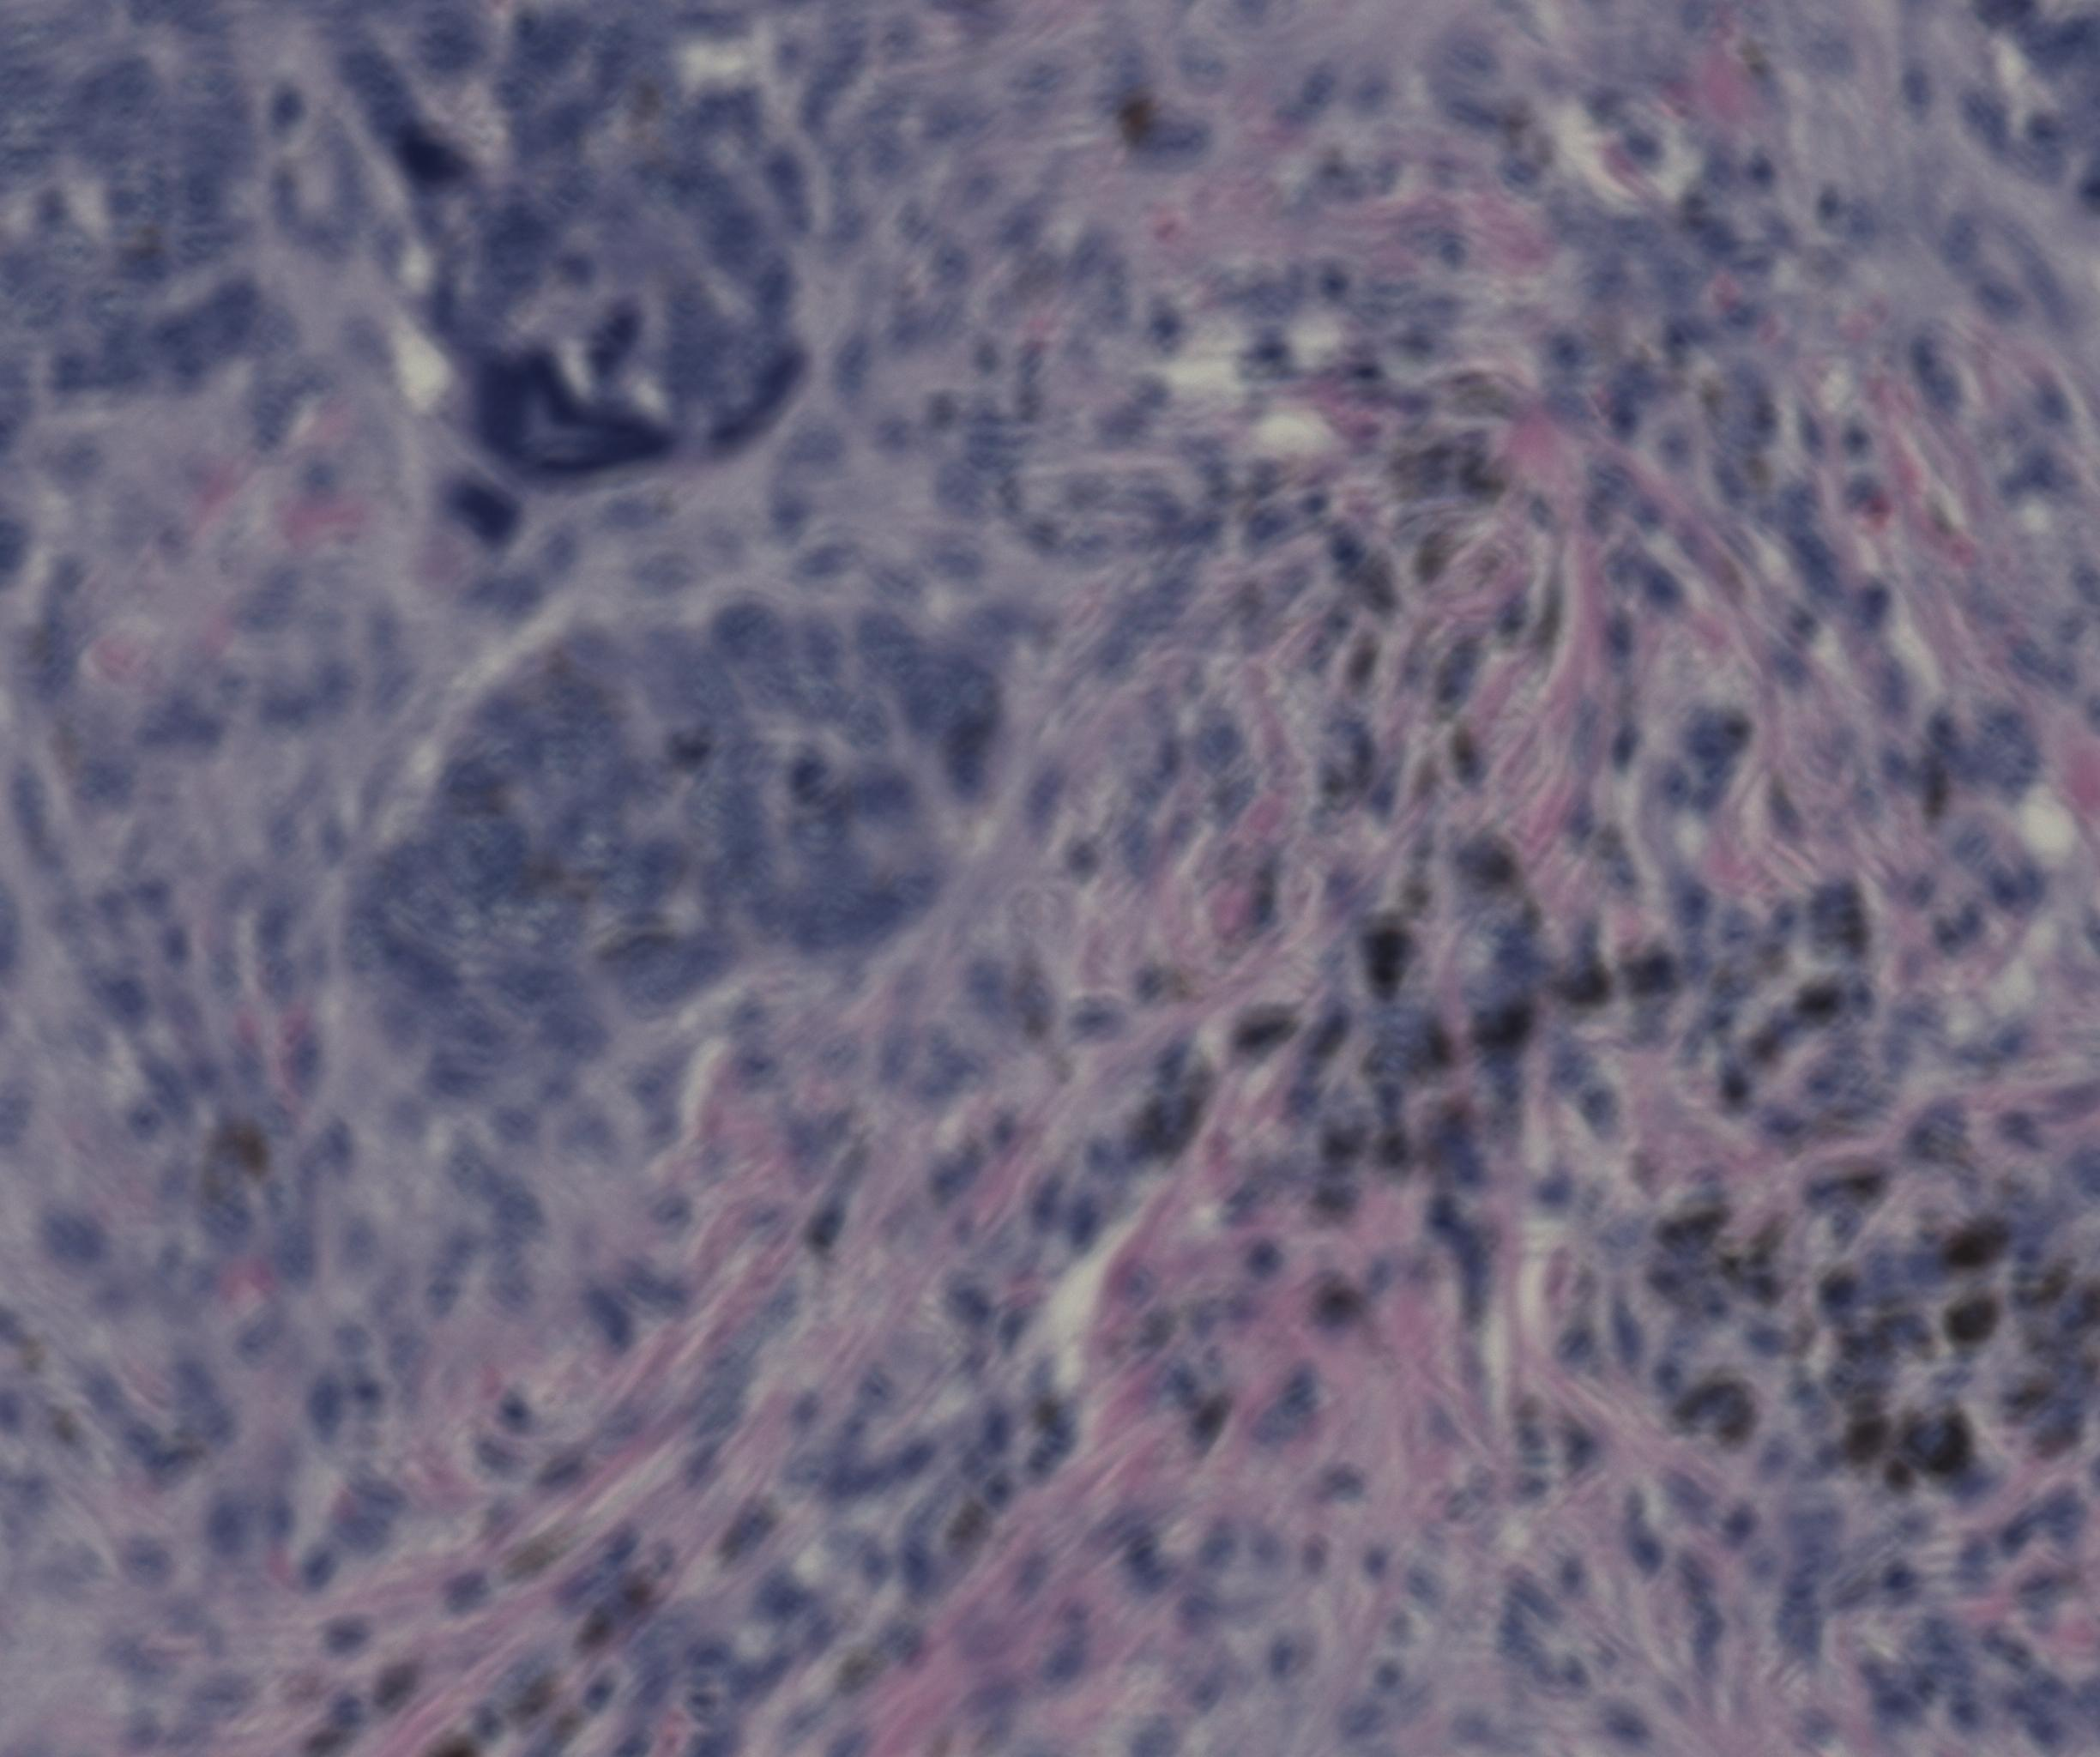
\includegraphics[width=1.0\linewidth]{my_folder/images/defocus6800.jpg}
%		\caption{}
%		\label{fig:defocus-2700}
%	\end{subfigure}
%	\hfill
%	\begin{subfigure}[t]{0.45\linewidth}
%		\centering
%		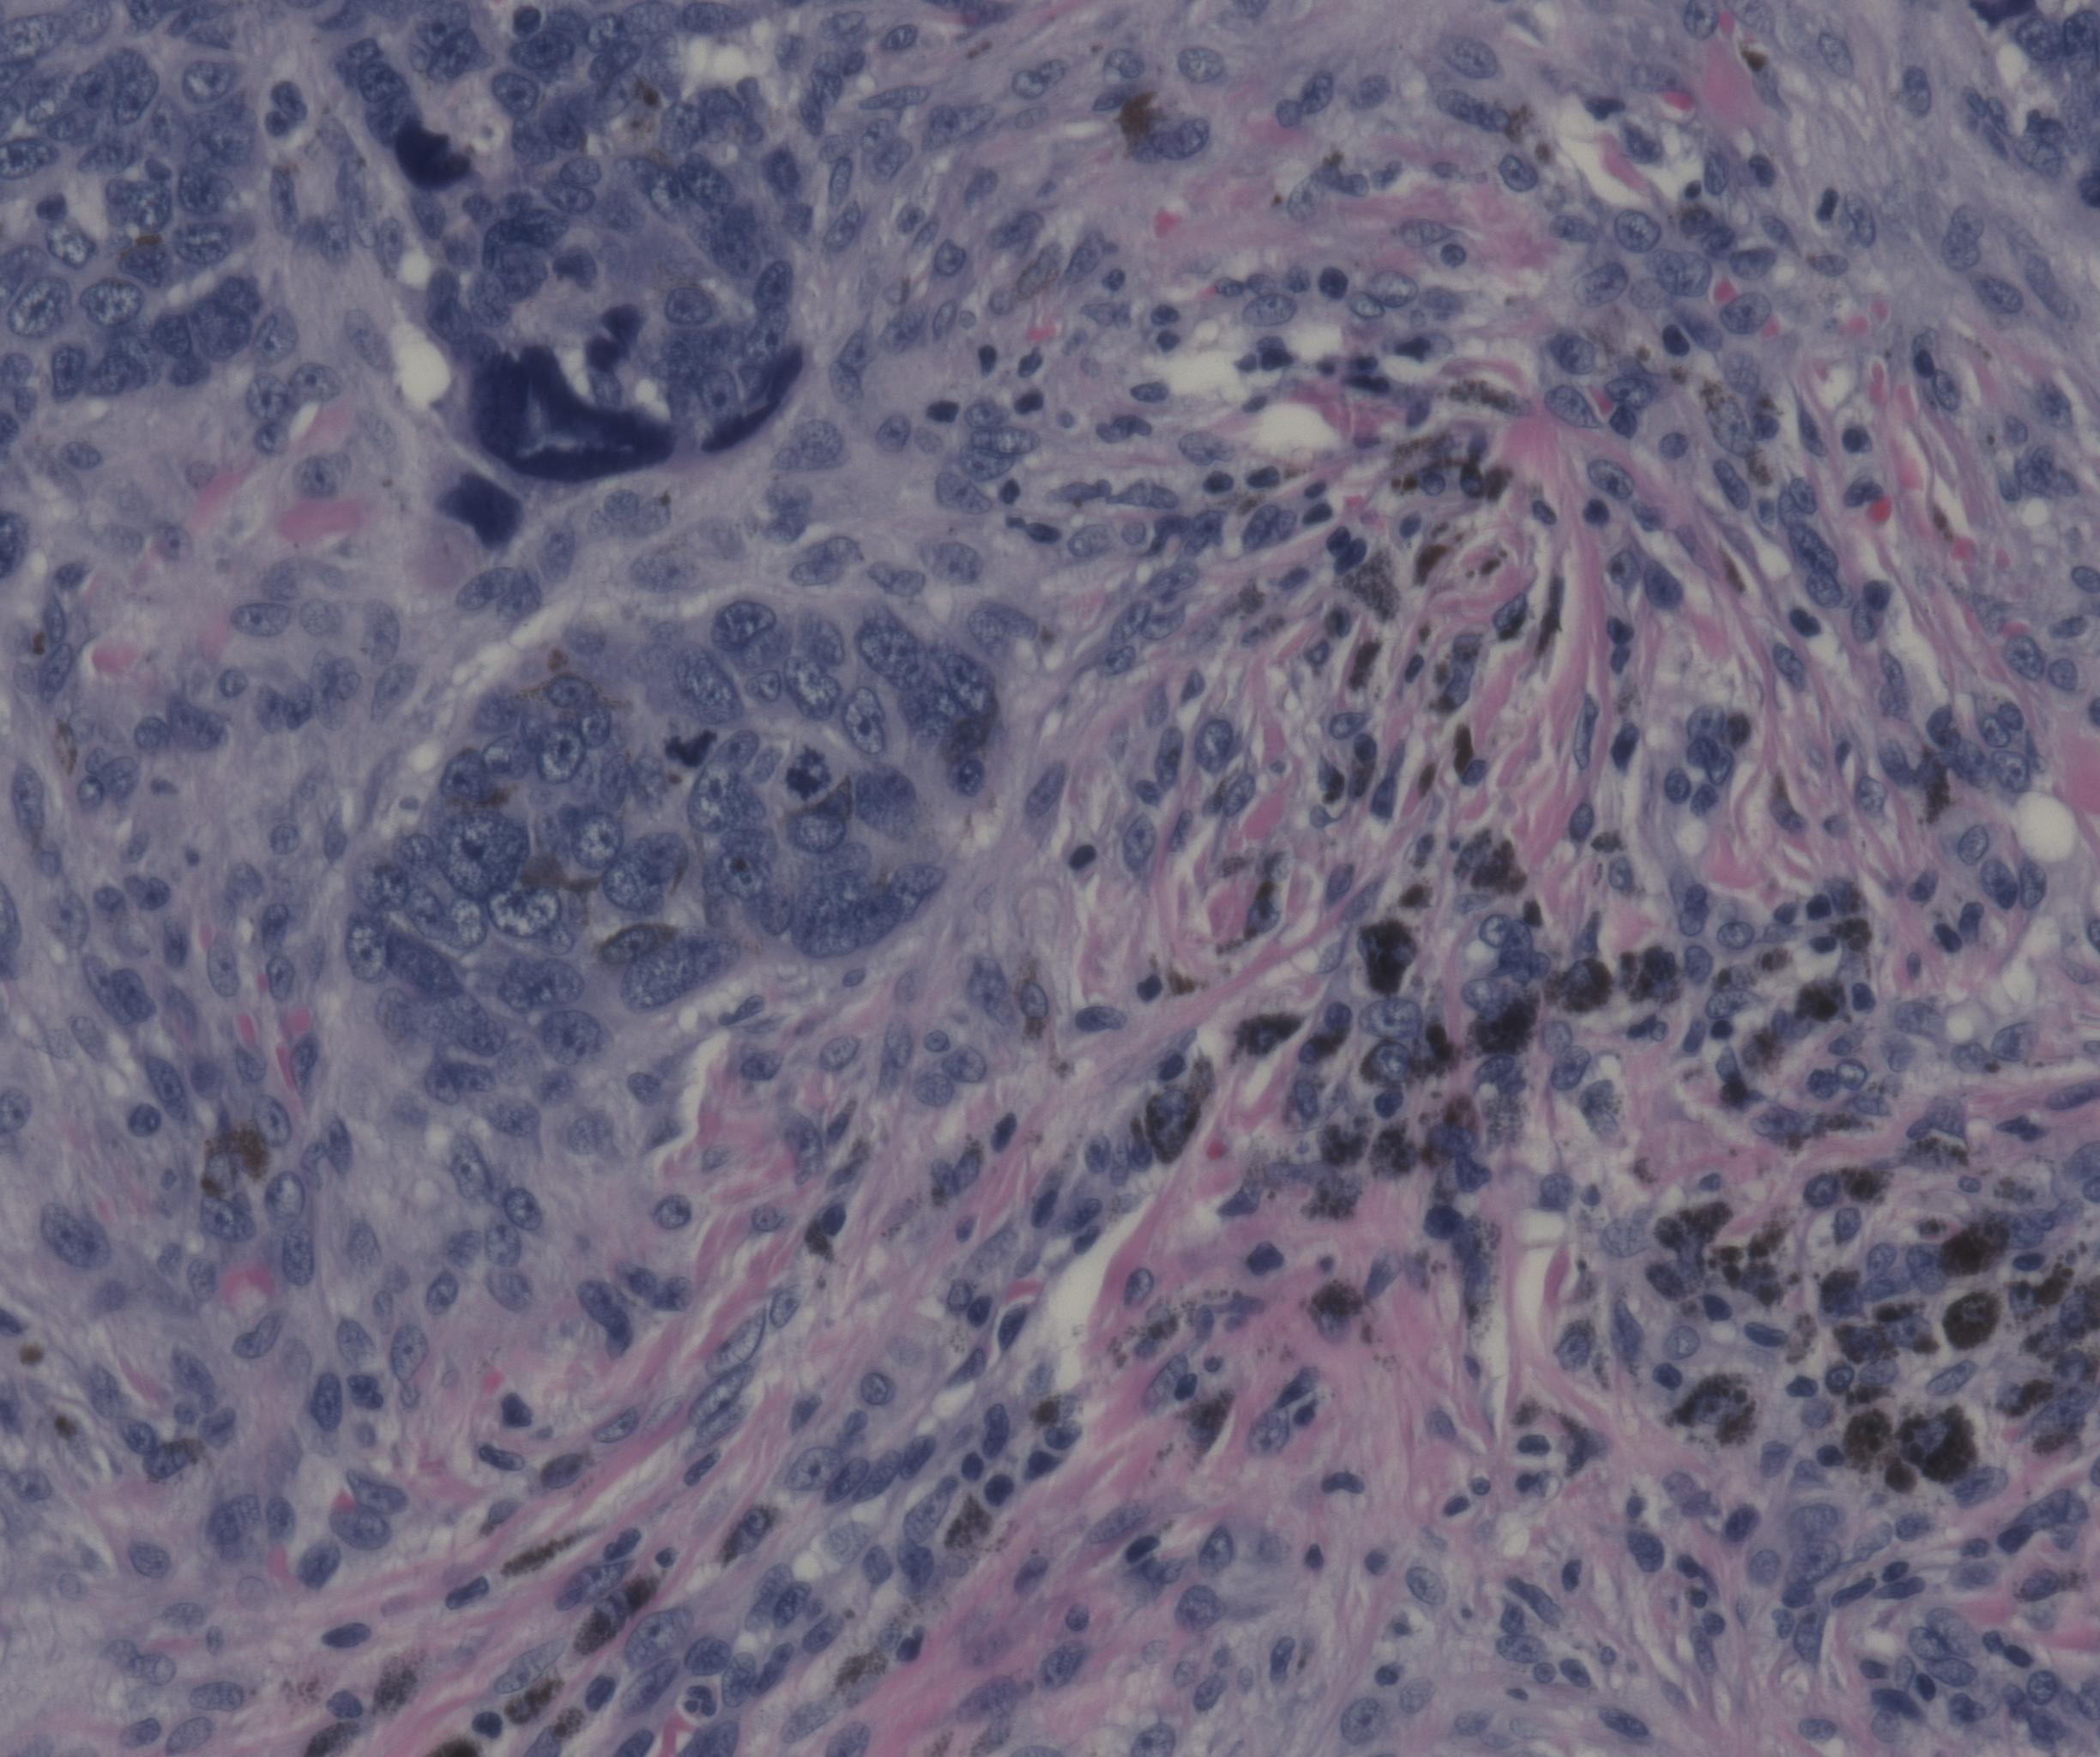
\includegraphics[width=1.0\linewidth]{my_folder/images/defocus-200.jpg}
%		\caption{}
%		\label{fig:defocus-200}
%	\end{subfigure}
%	\caption{Примеры работы алгоритма: {\itshape a} --- до фокусировки; {\itshape b} --- после фокусировки}
%	\label{fig:Result_example}
%\end{figure}

\begin{table}[!htbp]
	\centering
	\small
	\begin{tabular}{|m{3cm}<{\centering}|m{3cm}<{\centering}|m{3cm}<{\centering}|m{3cm}<{\centering}|m{3cm}<{\centering}|}
		\hline
		Метод& Время расчета одного смещения, мс & Ошибка, мкм & Число перемещений камеры & Общее время, мс \\\hline
		Контрастный автофокус & 29.0 & 6.3 & 13.4 & 1058.6\\\hline
		Метод анализа резкости & 27.5 & 5.2 & 11.2 & 871.4 \\\hline
		Нейросеть (CPU) & 81.7 & \multirow{2}{*}{\textbf{0.3}} & \multirow{2}{*}{\textbf{1}} & 131.7 \\\cline{1-2} \cline{5-5}
		Нейросеть (GPU) & \textbf{37.0} &  &  & 87.0 \\\hline
	\end{tabular}
	\caption{Сравнение классических методов и предлагаемой нейронной сети}
	\label{tab:Comparison_FocuesNet}
\end{table}

Решение на основе глубокого обучения также оказывается более устойчивым к шуму. Это свойство достигается за счет использования сверточных слоев. На \firef{fig:noise_example} изображены качественный снимок и его измененная версия, на которую добавлены шумы, распределенные по Гауссу и Пуассону. Ошибка в определении дистанции до фокальной плоскости в таком случае варьировалась в диапазоне $1.5-2.5$ мкм, что все еще меньше, чем у классических методов даже на нешумных снимках.

\begin{figure}[!htbp]
	\begin{subfigure}[t]{0.45\linewidth}
			\centering
			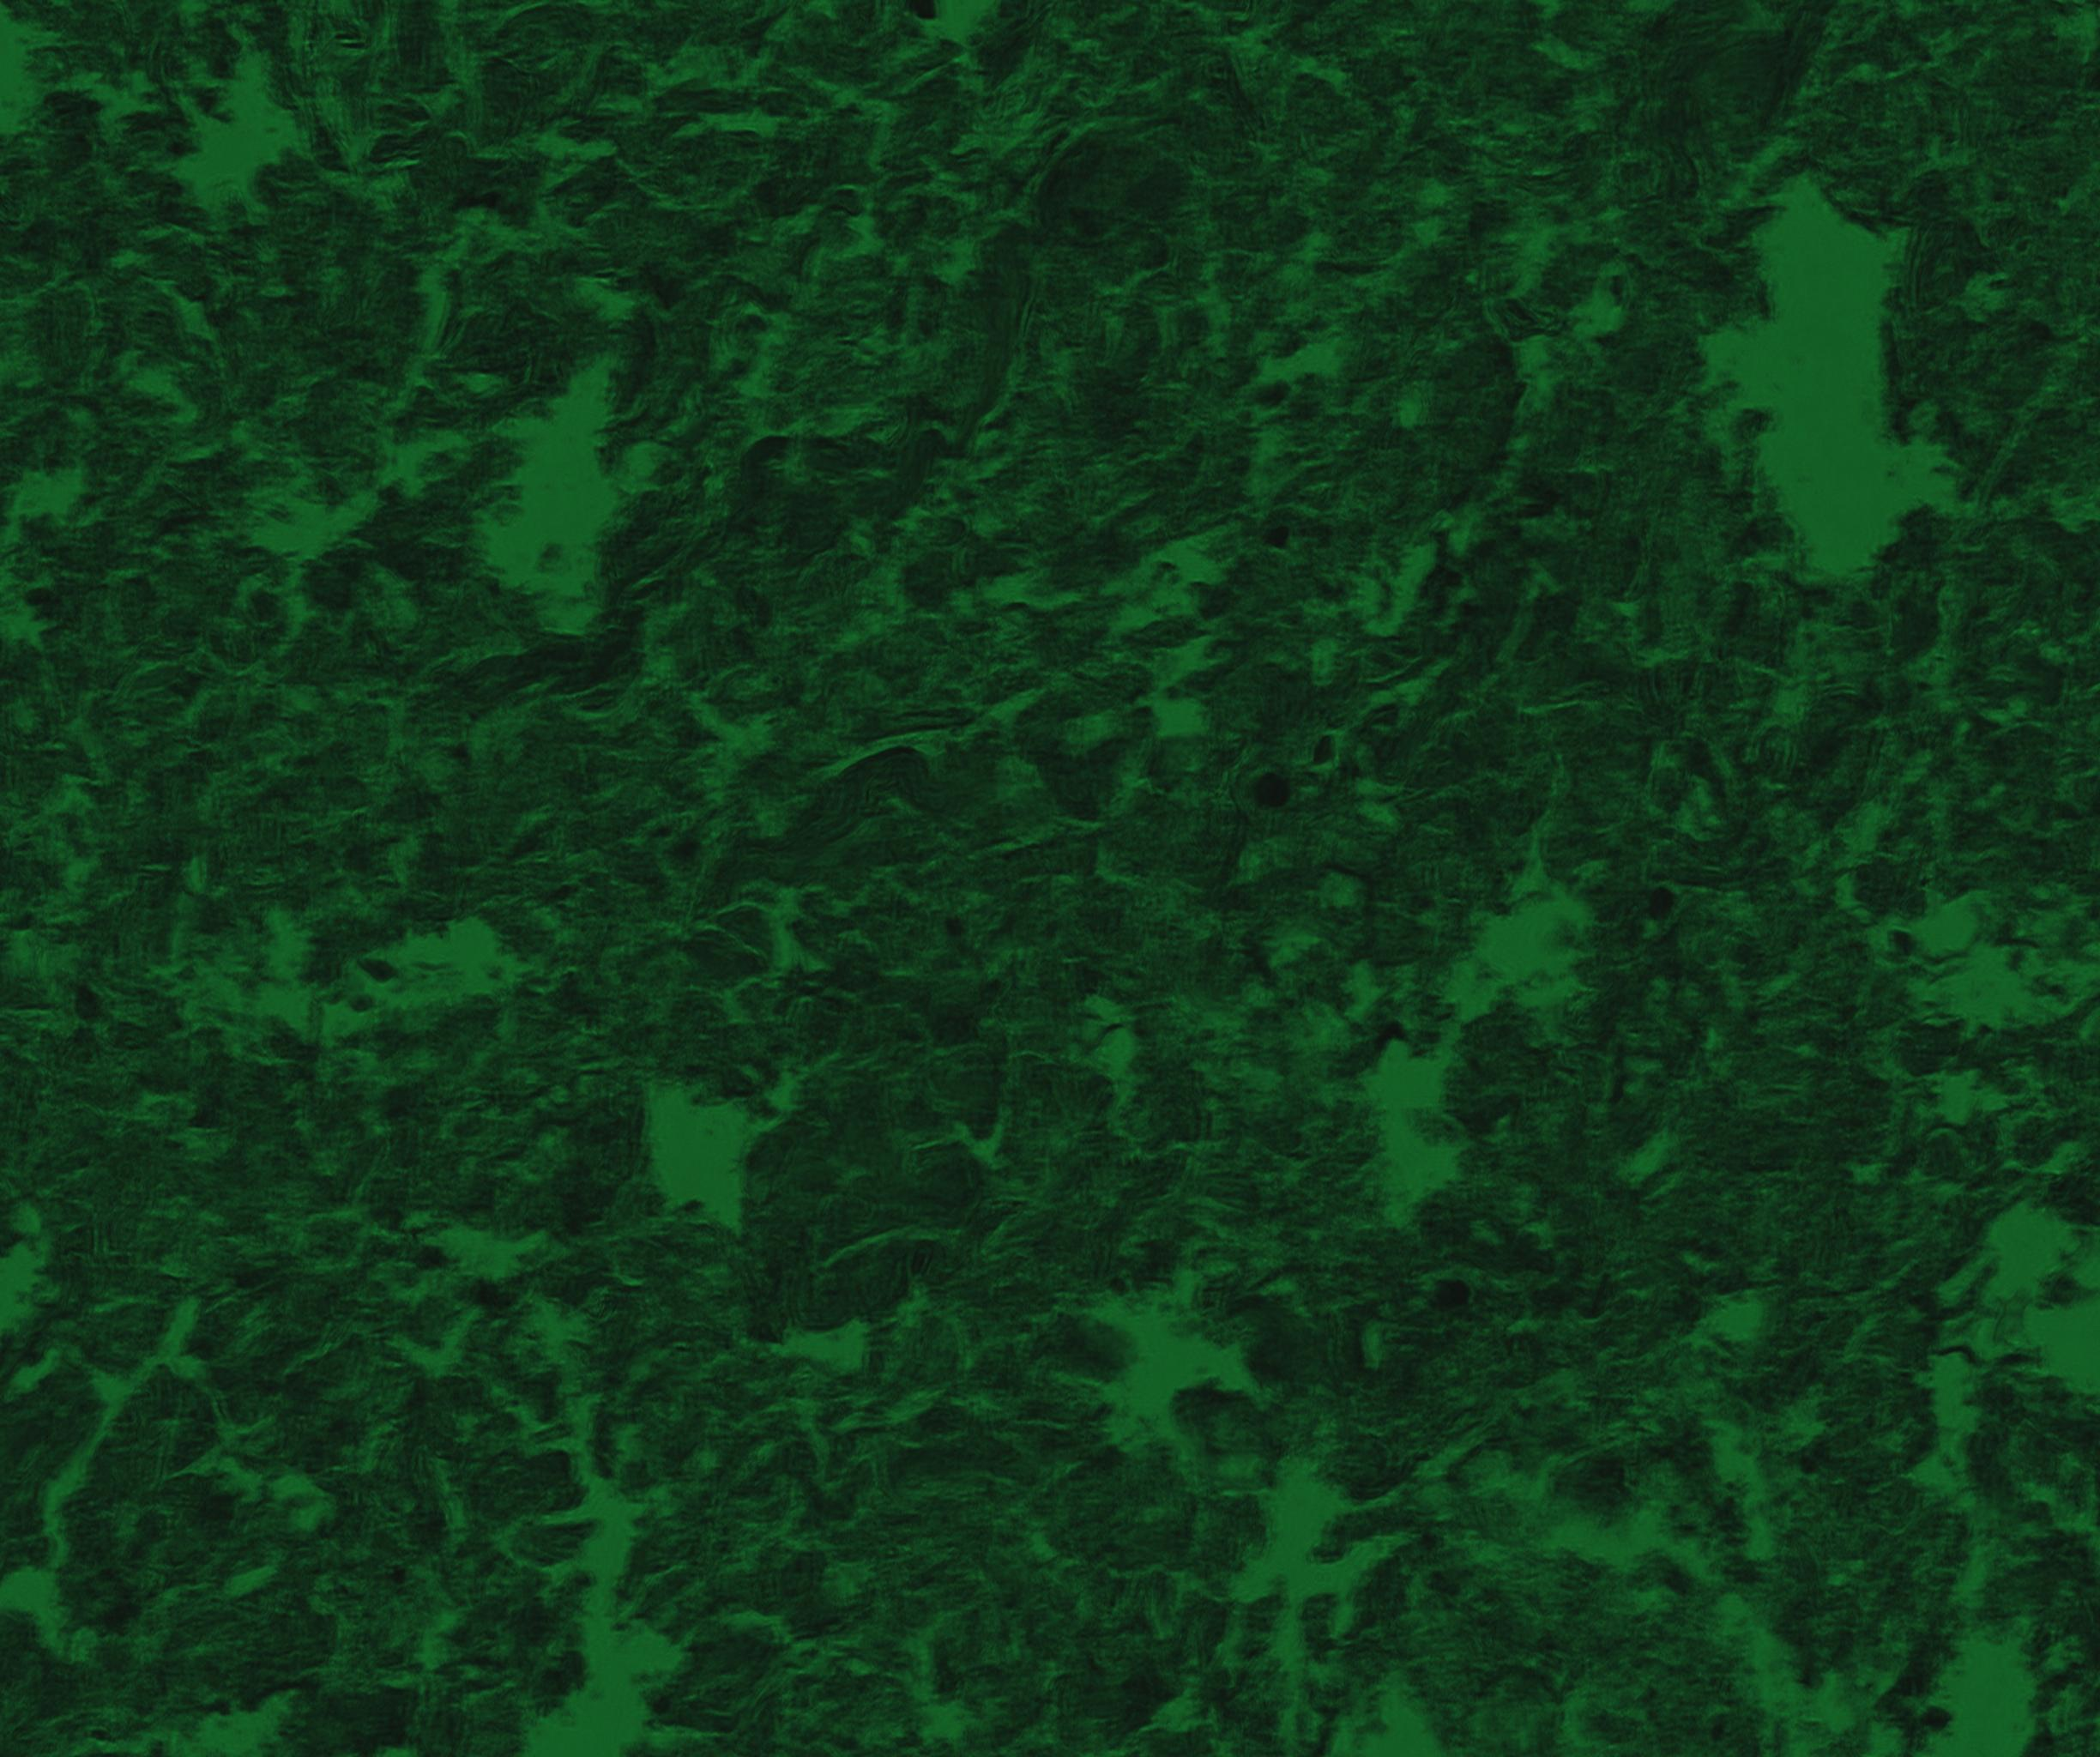
\includegraphics[width=1.0\linewidth]{my_folder/images/clear.jpg}
			\caption{}
			\label{fig:clear}
		\end{subfigure}
	\hfill
	\begin{subfigure}[t]{0.45\linewidth}
			\centering
			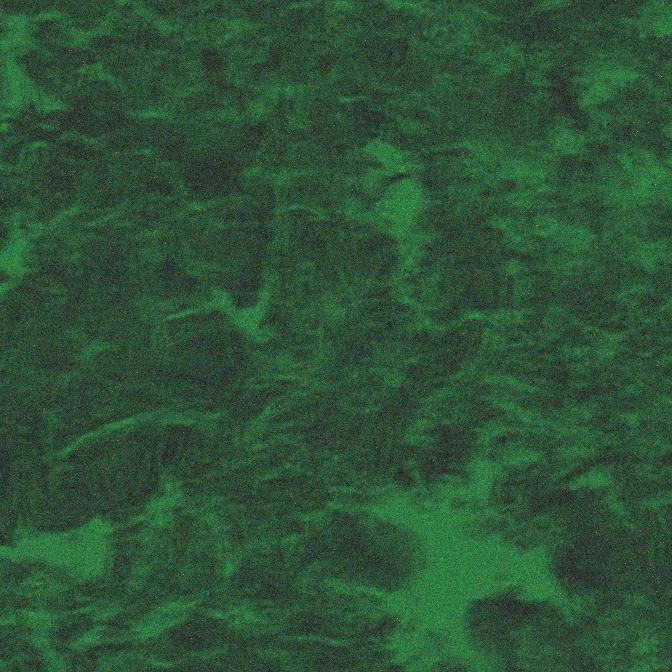
\includegraphics[width=1.0\linewidth]{my_folder/images/noisy.jpg}
			\caption{}
			\label{fig:noisy}
		\end{subfigure}
	\caption{Добавление шума: {\itshape a} --- чистый снимок; {\itshape b} --- зашумленный снимок}
	\label{fig:noise_example}
\end{figure}

%% Вспомогательные команды - Additional commands
%
%\newpage % принудительное начало с новой страницы, использовать только в конце раздела
%\clearpage % осуществляется пакетом <<placeins>> в пределах секций
%\newpage\leavevmode\thispagestyle{empty}\newpage % 100 % начало новой страницы